
\section{Context/Problem Statement} \label{sec:context}
This section further details a centralized architecture as well as its desirable features (synergy, reconfigurability) and its induced penalty (performance bottlenecks). 
Managing access control policies is one of the most challenging issues faced by organizations. Frequent changes in policy-based systems may be required to meet business needs. 
A policy-based system has to handle some specific requirements such as role swapping when employees are given temporary assignments, as well as changes in the policies and procedures, 
new assets, users and job positions in the organization.

\subsection{Centralization of Architectures}
To enable high reconfigurability, an access control policy is traditionally modeled, analyzed, and implemented as a separate component 
encapsulated in a PDP. This separation leads to the centralized architecture presented in Figure \ref{pep-pdp}, in which one single PDP is responsible for granting/denying the accesses that are requested. 
This centralized architecture is a simple solution to easily handle changes in policy-based systems by enabling the policy author 
to directly change policies on the single PDP. The separation between the PEP and the PDP simplifies policy management across many heterogeneous systems and limits
potential risks arising from incorrect policy implementation or maintenance, when the policy is hardcoded inside the business logic.
\begin{figure}[!h]
\begin{center}
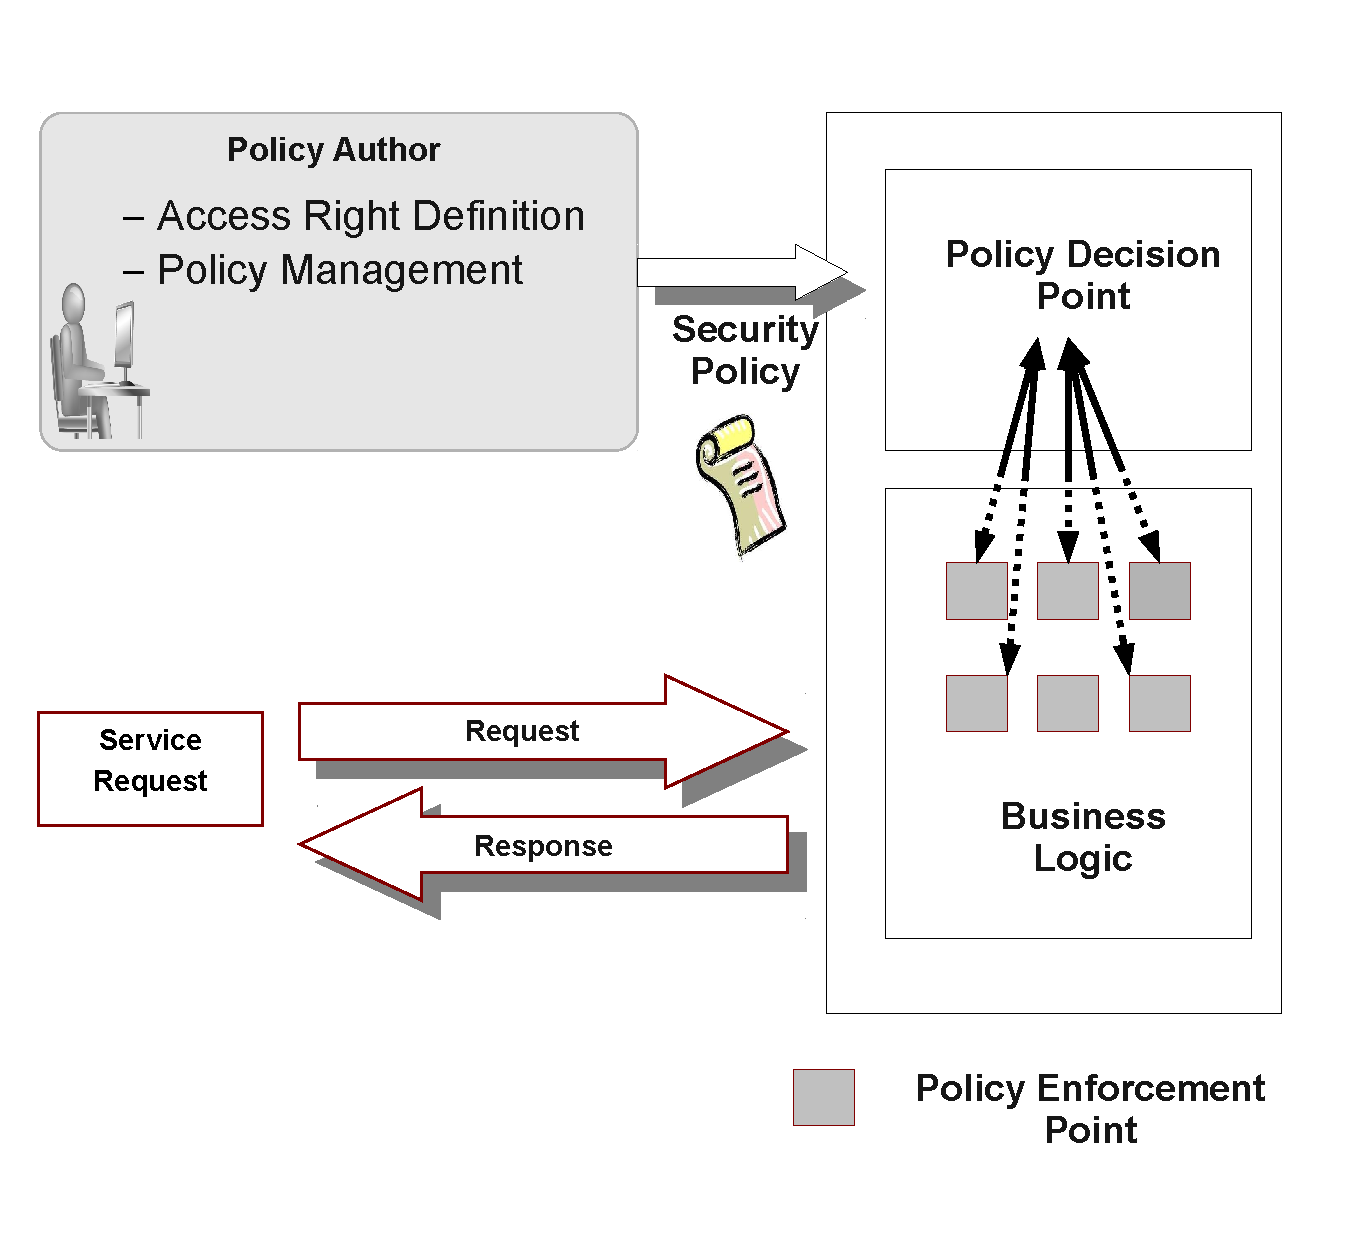
\includegraphics[width=9cm, height=8cm]{business-logic}
\caption{Access Control Request Evaluation}
\label{pep-pdp}
\end{center}
\end{figure}
\subsection{Centralization: A Threat for Performance}
In such a centralized system, when a service regulated by an access control policy, requires an access to some resources in the system, the PEP calls the PDP to 
retrieve an authorization decision based on the policy encapsulated in the PDP. This authorization decision is made through the evaluation of rules in the policy. 
Subsequently, an authorization decision (permit/deny) is returned to the PEP. When a huge number of access requests are sent by the PEP to the PDP, two bottlenecks cause a degradation of performance:
\begin{itemize}
 \item all the access requests have to be managed through the same input channel of the PDP. 
 \item the centralized PDP computes an access request by searching which rule is applicable among all the rules that the encapsulated policy contains.
\end{itemize}

The execution time for evaluating a request is thus strongly related to
\begin{itemize} 
\item the number of rules that the PDP contains as well as the order of the rules \cite{clustering}.
\item the workload (the number of requests that have to be managed by the system).
\end{itemize}
The execution time to evaluate a request depends on the size (number of rules) of the policy that the PDP encapsulates. For a given policy size, the execution time  to evaluate
 requests increases linearly with the workload the (number of requests). 
Our hypothesis 1 is that the more rules a policy contains, the higher the slope of the execution time with an increasing workloads. 
 \textit{Hypothesis 1} validity is discussed in Section \ref{sec:experiment}.
As a consequence, one possibility to improve performance consists in splitting the centralized PDP into PDPs with smaller policy sizes. 
It is worth to mention that in this paper, we keep the same input channel in the decentralized architecture. In such setting, we do not need to change the PEP code that is calling 
the PDP. In fact, to set a specific input channel for each PEP, we need to change the code, so that each PEP calls directly its PDP, however, in this work, we consider the system as
 a black box for sake of simplicity and scalability.  


\subsection{Centralization: PEPs and PDP Synergy}
Centralization offers a desirable feature by simplifying the routing of requests to the right PDP. 
Figure \ref{model} illustrates the model of the access control architecture. In this model, a set of business processes, which comply to users' needs, are encapsulated 
in a given business logic, which is enforced by multiple PEPs. Conceptually, the decision is decoupled from the enforcement and involves a decision making process in which each PEP 
interacts with one single PDP. The key point concerns the cardinality linking PEPs to the PDP. While a PDP is potentially linked to many PEPs, any PEP is strictly linked to exactly one 
PDP (which is unique in the centralized model). 
Since there is only one PDP, the requests are all routed to this unique PDP. No particular treatment is required to map a given PEP in the business logic to 
the corresponding PDP, embedding the requested rules. Another advantage of this many-to-one association is the clear traceability between what has been specified by the 
policy at the decision level and the internal security mechanisms enforcing this policy at the business logic level. In such setting, 
when access control policies are updated or removed, the related PEPs can be easily located, updated and removed. Thus the application is updated synchronously 
with the policy changes. We call this desirable property \textit{synergy} of the access control architecture: an access control architecture is said to be \textit{synergic} if any PEP always sends 
its requests to the same PDP. 
As a consequence, splitting the centralized PDP into PDPs of smaller policies sizes may break this 'synergy' since calls issued by PEPs can be handled by several PDPs. 
In this work, we consider various splitting criteria to transform a centralized PDP into PDPs with smaller policies size. 
Our \textit{hypothesis 2} is with comparable PDP policies sizes, the overall system will be more performant when the architecture is synergic. This hypothesis is investigated in 
Section \ref{sec:experiment}.

\subsection{Tradeoff for refactoring }

As a synthesis for this section, the following facts are taken into account:
\begin{itemize}
 \item Access control architectures are centralized with a unique PDP.
\item Centralization eases reconfiguration of an access control policy.
\item Centralization threatens performance.
\item Direct mapping from any PEP to only one PDP makes the access control architecture 'synergic'.
\item A synergic system facilitates PEP request routing and eases policy maintenance.

\end{itemize}

The goal our our work is to propose systematic ways to improve performance by refactoring the centralized model into a decentralized version, with multiple PDPs. The resulting
 architecture must have an equivalent behaviour and should not impact the desirable properties of the centralized model, namely reconfigurability and synergy. 
Automating the transformation from a centralized to a decentralized architecture is required to preserve reconfigurability. With automation, we can still reconfigure the centralized policy, 
and then automatically refactor the architecture. Automated refactoring is thus a viable solution for providing high reconfigurability.  
However, refactoring the architecture by splitting the centralized PDP into smaller one may break the initial synergy. This phenomenon is studied in the empirical study of Section 
\ref{sec:experiment} together with \textit{hypothesis 2}. In the next section, we give an overview of XACML language since it is the standard language used in this paper to implement a PDP.


\begin{figure}[!h]
\begin{center}
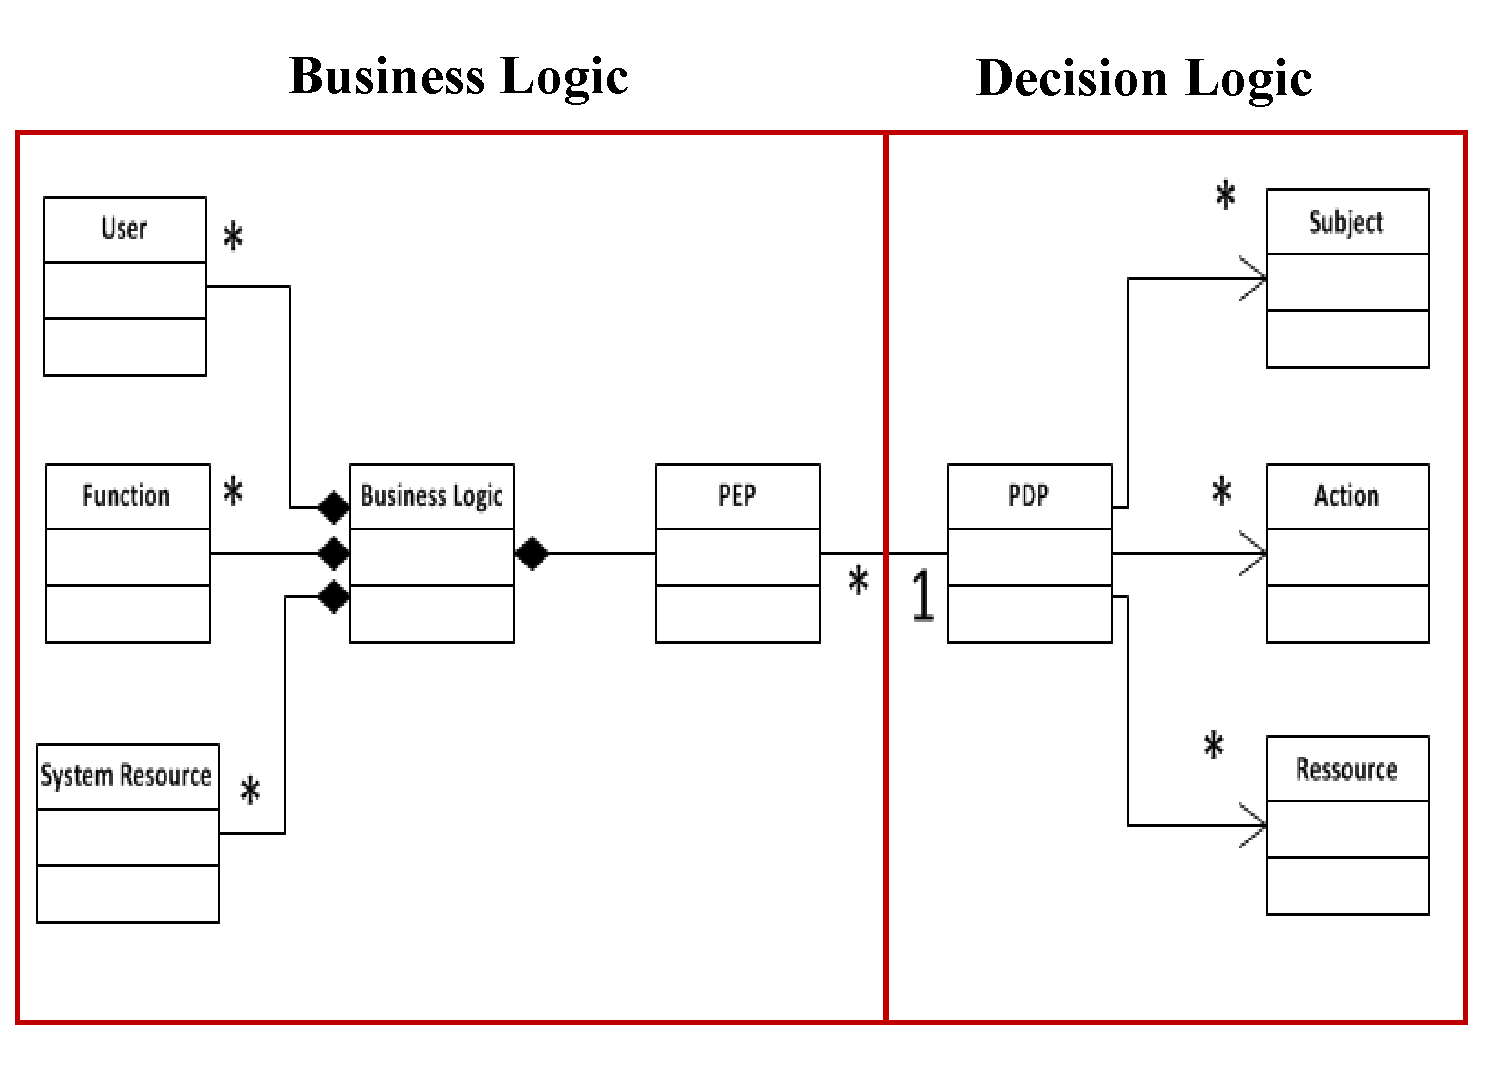
\includegraphics[height=5.5cm,width=8.5cm]{model}
\caption{Access Control Model}
\label{model}
\end{center}
\end{figure}

\subsection{XACML Policies and Performance Issues}
In this paper, we focus on access control policies specified in the eXtensible Access Control Modeling Language (XACML) \cite{sunxacml}.
XA-CML is an XML-based standard policy specification language that defines a syntax of access control policies and
requests/responses. \\XACML enables policy authors to externalize access control policies for the sake of interoperability since access control policies can be designed 
independently from the underlying programming language or platform. Such flexibility enables to easily update access control policies to comply with new requirements.
An XACML policy is constructed as follows.
A \CodeIn{policy set} element consists of a sequence of \CodeIn{policy} elements, a combining algorithm, and
a \CodeIn{policy target} element. A \CodeIn{policy} element is expressed through a \CodeIn{target}, a set of \CodeIn{rules}, and a rule combining algorithm. 
A \CodeIn{target} element consists of the set of resources, subjects, and actions to which a rule is applicable. A \CodeIn{rule} consists of a 
\CodeIn{target} element, a \CodeIn{condition} element, and an \CodeIn{effect}. A \CodeIn{condition} element is a boolean expression that specifies the
environmental context (e.g., time and location restrictions) in which the rule applies.
Finally, an \CodeIn{effect} is the rule's authorization decision, which is either permit or deny.
Given a request, a PDP evaluates the request against the \CodeIn{rules} in the policy by matching resources, subjects and actions in the request.
More specifically, an XACML request encapsulates attributes, that define which subject requests to take action on which resource (e.g., subject Bob requests to borrow a book).
%This can be under/not a condition.
Given a request that satisfies \CodeIn{target} and \CodeIn{condition} elements in a rule, the rule's effect
is taken as the decision.
If the request does not satisfy \CodeIn{target} and \CodeIn{condition} elements in any rule, its response yields the ``NotApplicable'' decision.

When more than one rule is applicable to a request, the combining algorithm helps determine which rule's effect can be finally given as the decision for the request.
For example, given two rules that are applicable to the same request and provide different decisions,
the permit-overrides algorithm prioritizes a permit decision over the other decisions.
More precisely, when using the permit-overrides algorithm, the policy evaluation produces one of the following three decisions for a request: 

\begin{itemize}
\item Permit if at least one permit rule is applicable for the request.
\item Deny if no permit rule is applicable and at least one deny rule is applicable for a request.
\item NotApplicable if no rule is applicable for the request.
\end{itemize}

A \CodeIn{policy target} element describes what the policy applies to by referring to attributes of users, resources and actions.

Figure \ref{figur1} shows a simplified XACML policy that denies subject Bob to borrow a book.

%\fontsize{5}{5}
\begin{figure}[!h]
\begin{center}
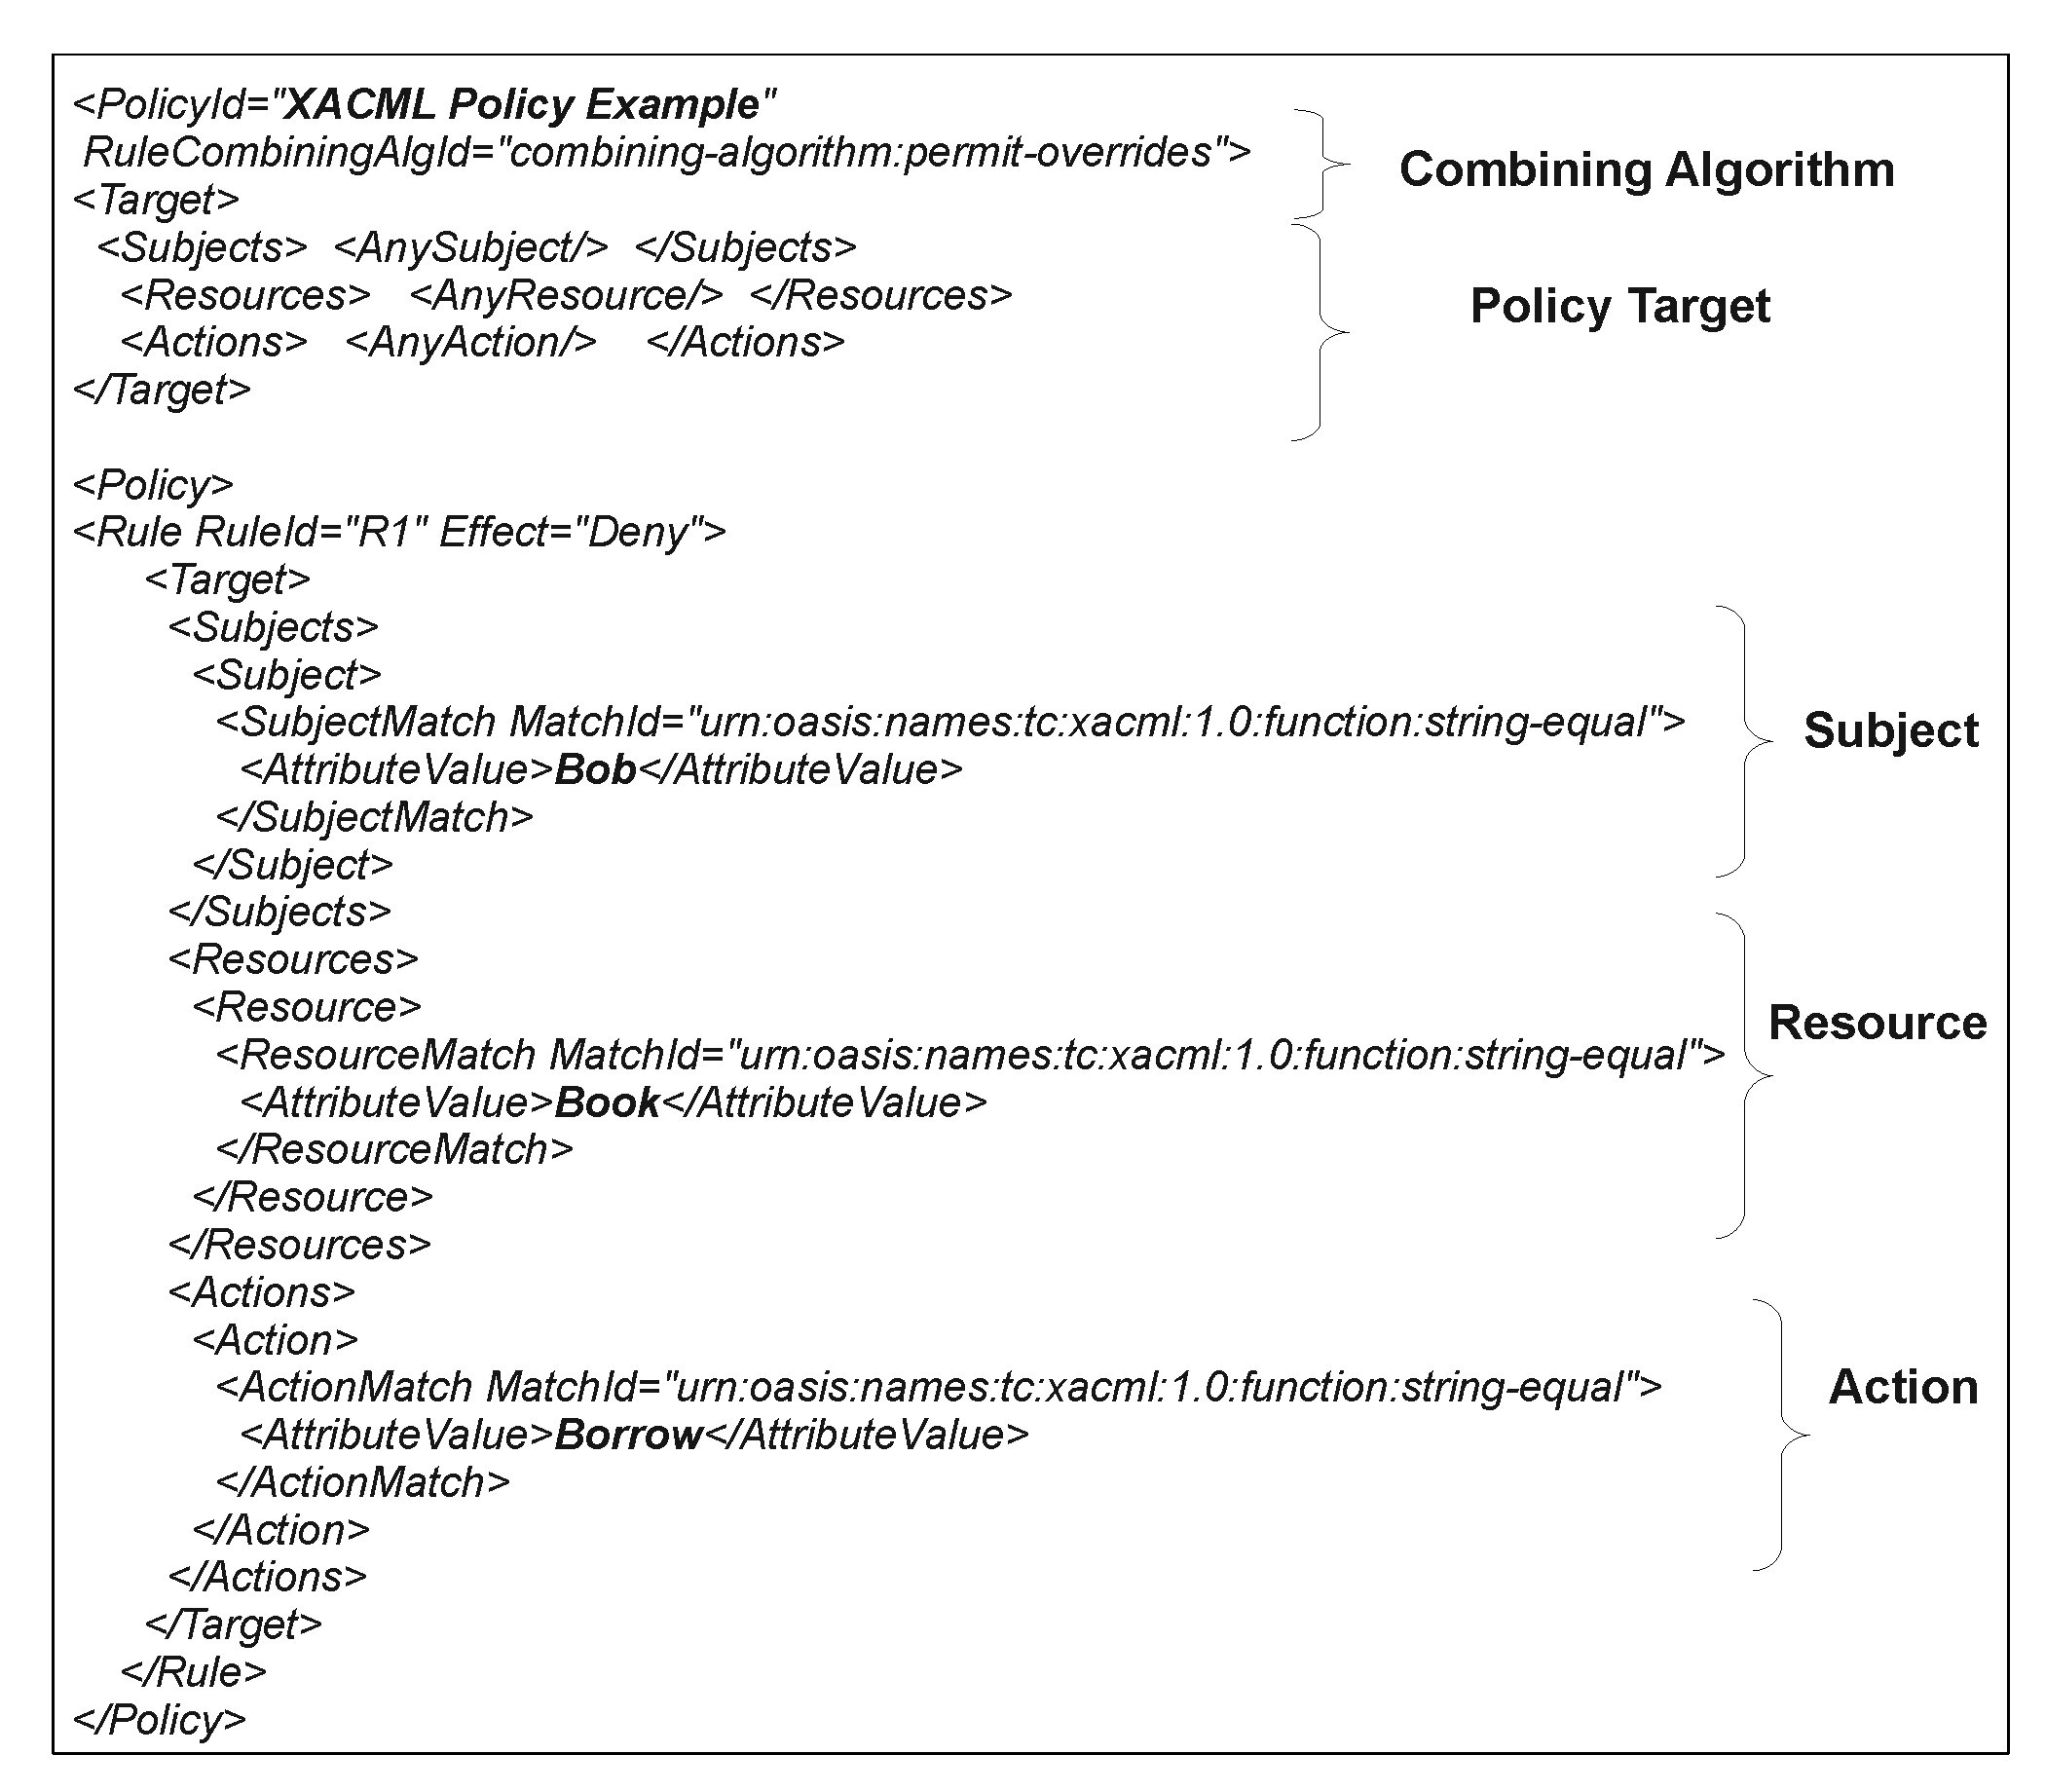
\includegraphics[width=8.6cm]{xacml}
\caption{XACML Policy Example}
\label{figur1}
\end{center}
\end{figure}


XACML policies becomes more complex when handling increasing complexity of organizations in terms of structure, relationships, activities, and access control requirements. In such a situation, a policy 
often consists of a large number of rules to specify policy behaviors for various resources, users, and actions in the organizations.
In policy-based systems, policy authors manage a centralized and a single PDP loaded with a single policy to govern all system resources. 
However, due to a large number of rules for evaluation, this centralization raises performance concerns related to request evaluation time for access control policies and may 
degrade the system efficiency and slow down the overall business processes. 

We present the following three main factors that may cause to degrade XACML request evaluation performance: 

\begin{itemize}
\item An XACML policy may contain various attribute elements including \CodeIn{target} elements. Retrieval of
attribute values in the \CodeIn{target} elements for request evaluation may increase the evaluation time.
\item A \CodeIn{policy set} consists of a set of policies. Given a request, a PDP determines the final authorization decision (i.e., effect) of 
the whole \CodeIn{policy set} after combining all the applicable rules' decisions for to the request.
Computing and combining applicable rules' decisions contribute to increasing the evaluation time.
\item \CodeIn{Condition} elements in rules can be complex because these elements are built from an arbitrary nesting of non-boolean functions and attributes. 
In such a situation, evaluating \CodeIn{condi-\\tion} elements may slow down request evaluation time.
\end{itemize}

